
\documentclass[brazilian]{ifsc-tcc}
%----------------------------------------------------------------------
\usepackage{float}
\usepackage{breakcites}
\usepackage[utf8]{inputenc}
\usepackage[T1]{fontenc}
\usepackage{graphicx,url}
\usepackage{graphics}
\usepackage{url}
\usepackage[explicit]{titlesec}
\usepackage[brazilian,hyperpageref]{backref}	 % Paginas com as citações na bibl
\usepackage[alf, abnt-etal-cite=1]{abntex2cite}			% Citações padrão ABNT
\usepackage{lipsum}

\usepackage{multirow}
\usepackage[table,xcdraw]{xcolor}
\usepackage{graphicx}


% \errorcontextlines\maxdimen
% informações do PDF
\makeatletter
\hypersetup{
     	%pagebackref=true,
	pdftitle={\@title}, 
	pdfauthor={\@author},
	pdfsubject={\imprimirpreambulo},
	pdfcreator={LaTeX with abnTeX2},
	pdfkeywords={abnt}{latex}{abntex}{abntex2}{trabalho acadêmico}, 
	colorlinks=true,       		% false: boxed links; true: colored links
    	linkcolor=black,          	% color of internal links
    	citecolor=blue,        		% color of links to bibliography
    	filecolor=magenta,      		% color of file links
	urlcolor=blue,
	bookmarksdepth=4
}

%----------------------------------------------------------------------
% Identificadores do trabalho
% Usados para preencher os elementos pré-textuais
\instituicao{Instituto Federal de Santa Catarina} % Opcional
\titulo{Software para Previsão de Partidas de Basquete usando Algoritmos Genéticos em Python}
\autor{Bernardo Pires Mesko, Grégori Sabel, João Vitor Waldrich, Rafael Guilherme Onesko}
\local{Gaspar, SC, Brasil} % Opcional 
\data{\today}
\orientador{Thiago Lipinski Paes, Dr.}
\coorientador{Rafael Silvano Ferreira Silva}

% \centro{}
% \programa{}
\tipotrabalho{Tese}
\preambulo{Projeto Integrador apresentado ao Curso Técnico Integrado em Informática do Campus Gaspar do Instituto Federal de Santa Catarina como requisito parcial para aprovação na unidade curricular Projeto Integrador I.}
%\preambulo{Trabalho de Conclusão de Curso apresentado ao Curso Superior de Tecnologia em Análise e Desenvolvimento de Sistemas como requisito parcial para obtenção do grau de Tecnólogo em  Análise e Desenvolvimento de Sistemas.}

\begin{document}

\pretextual%
\imprimircapa%
\imprimirfolhaderosto*%
\clearpage
\imprimirfichacatalografica%

\clearpage

\begin{resumo}[resumo]

O basquete é provavelmente um dos esportes mais populares da atualidade. Toda essa fama é acompanhada de um mercado bastante lucrativo, que movimenta bilhões de dólares todos os anos. Os jogos de basquete não afetam somente seus times e outras organizações diretamente envolvidas com as partidas; afeta todo um contexto social, desde torcedores, empresas, dentre vários outros. Dentre todo esse nicho temos também as pessoas pertencentes ao crescente mercado de apostas esportivas. % contextualização
Uma grande demanda desse ramo é a existência de algum método que consiga prever, com segurança e da melhor forma, resultados de partidas: um problema com uma complexidade grande o suficiente para até mesmo recentemente não poder ser resolvido de maneira simples. %problema
Com a grande quantidade de ferramentas disponíveis, foi preciso avaliar quais linguagens e metodologias seriam as mais adequadas para o projeto e, com as informações disponíveis. Depois de uma vasta pesquisa foi definido a linguagem de programação Python como a base do projeto devido a sua simplicidade e agilidade, integrando-a com algoritmos de web scraping para coleta de dados.
Este trabalho tem como objetivo o desenvolvimento de uma estratégia própria para a previsão de resultados de partidas, e espera que possam ser usados algoritmos genéticos para testar o impacto de diversos aspectos de um time para a inferência de seu desempenho no primeiro quarto tempo de uma partida na NBA no \textit{software} desenvolvido. \newline

\noindent \textbf{Palavras-chave: Basquete. Previsão. Algoritmo Genético. Python.}

\end{resumo}
\begin{resumo}[Abstract]
\begin{otherlanguage*}{english}
%hora de encarnar o english speaker
Basketball is probably one of present day's most popular sports. All this fame is surrounded by a very lucrative market, which trades billions of dollars every year. The Basketball matches don't affect only their teams and other directly involved organizations with them; it concerns a whole social context, from fans of the sport, to businesses, between several others. Inside this niche we also have people belonging to the growing market of sports
One big demand of this branch is the existence of some method able to predict, with security and by the best possible manner, match results: a problem with a big enough complexity for it not to be solved in a simple way until recently.
With the sheer amount of available tools, it was necessary to determine which languages and methodologies would be the most adequate for the project. After a wide search it was defined that the Python programming language would be the basis for the system, due to its simplicity and agility, integrating it with web scraping algorithms for data collection.
This research project has as its objective the development of a proprietary strategy for match results prediction, and it is hoped that genetic algorithms will be used in the developed software for testing the impact of several aspects of a team on the inference of its performance in the first quarter time of a NBA match.

\noindent \textbf{Keywords: Basketball. Prediction. Genetic algorithm. Python,}

\end{otherlanguage*}
\end{resumo}


% ---
% inserir lista de ilustrações
% ---
\pdfbookmark[0]{\listfigurename}{lof}
\listoffigures*
\cleardoublepage
% ---

% ---
% inserir lista de tabelas
% ---
\pdfbookmark[0]{\listtablename}{lot}
\listoftables*
\cleardoublepage
% ---

% ---
% inserir lista de simbolos
% ---


% ---
% inserir lista de abreviaturas
% ---
\listadeabreviaturas
\cleardoublepage

% ---
% inserir sumário
% ---
\tableofcontents*
\cleardoublepage

\tipotrabalho{Trabalho de Conclusão de Curso}
      
\textual

% ---
% inserir definição das siglas e símbolos
% ---
\simbolo{$bb_i$}{Basic block i}


\simbolo{}{}

\sigla{IFSC}{Instituto Federal de Santa Catarina}
\sigla{NBA}{National Basketball Association}
\sigla{IA}{Inteligência Artificial}
\sigla{HTML}{Hypertext Markup Language}
\sigla{GTK}{GIMP Toolkit}
\sigla{GIMP}{GNU Image Manipulation Program}
\sigla{GNOME}{GNU Network Object Model Environment}
\sigla{NBB}{Novo Basquete Brasil}
\sigla{TCC}{Trabalho de Conclusão de Curso}
\sigla{CSV}{Comma Separated Values}
\sigla{AG}{Algoritmo Genético}
\sigla{RF}{Requisito Funcional}
\sigla{RNF}{Requisito Não Funcional}

\sigla{}{}

 

\chapter{INTRODUÇÃO}

A \textit{National Basketball Association} (NBA) é uma das principais ligas de basquetebol profissional da América do Norte, e de acordo com a \textit{Harvard Sports Analysis} é um dos campeonatos desse esporte com maior paridade, ou seja, os times dessa liga possuem um nível de habilidade muito semelhante, o que por sua vez acarreta competições mais justas \cite{paridade-basquete-harvard}. Junto aos diversos fãs do esporte e acompanhadores da liga surge também uma grande quantidade de receita gerada: em torno de US\$ 8 bilhões na temporada de 2019 \cite{nba-revenue-2019}.

O mercado de apostas esportivas, outro setor importante, movimenta anualmente centenas de bilhões de dólares em todo o mundo. Esse fato atrai diversas pessoas interessadas em lucrar com este mercado. O site Terra estima que 2 bilhões de reais são movimentados por ano somente no Brasil, por exemplo \cite{dados-dinheiro-terra}. 

Embora esse mercado tenha um grande potencial para a movimentação da economia, o Brasil se encontra relativamente atrasado neste setor. A regulamentação brasileira de apostas esteve em hiato por muito tempo \cite{tcc-regulamentacao-apostas}, até a criação da lei nº 13.756/18, que cria a definição de apostas de quota fixa (uma categoria que engloba as apostas esportivas) num contexto legislativo, e prevê um prazo de 2 anos para sua regulação pelo Ministério da Fazenda \cite{lei1375618}.

Há uma demanda muito grande de métodos confiáveis de previsão de resultados de partidas. Com esse intuito, diversas metodologias vêm sendo criadas, como a previsão com base em estatísticas prévias \cite{modelagem-estatistica-futebol} ou com mineração de dados \cite{Predicao-de-playoff-com-mineracao-de-dados}, por exemplo. De forma geral, partidas de basquete envolvem muitas variáveis, e isso as torna difíceis de prever com segurança, ainda mais em uma liga tão competitiva quanto a NBA.

Unificando o mundo da NBA com o das apostas esportivas percebe-se que, além de uma boa previsão de resultados, é preciso levar em consideração as chamadas \textit{odds}, as probabilidades de cada resultado ocorrer, que estão diretamente relacionadas ao valor pago pelas casas de aposta em caso de acerto. Configura-se, então, grande desafio: desenvolver uma solução que seja capaz de prever resultados e que, além disso, seja rentável a curto, médio ou longo prazo. 

Deste modo, o presente trabalho tem como objetivo geral a criação de uma solução relativamente confiável, que emprega estatísticas pregressas em conjunto com o método computacional de algoritmos genéticos para fornecer indicações de vitória em partidas de basquete. O escopo inicial do trabalho ficará limitado apenas a times participantes da NBA, e a validação do trabalho, por sua vez, será feita a partir da comparação das previsões de resultados de partidas passadas feitas pelo programa com seus reais resultados. O programa também irá prever resultados de jogos futuros, os quais, à medida que acontecerem, servirão de indicador de sua precisão.


\section{OBJETIVOS}
Nessa seção serão mostrados o objetivo geral e os objetivos específicos do projeto proposto.

\subsection{Objetivo geral}
Desenvolver uma aplicação que analisa dados de jogos da NBA e que com eles tente prever o time vencedor do primeiro quarto tempo em uma partida.

\subsection{Objetivos específicos}

\begin{enumerate}
\item Coletar dados necessários para o programa sendo através de Web scraping;
\item Utilizar IA para formular uma relação entre esses dados e;
\item Apresentar os resultados da previsão de forma clara e precisa.
\end{enumerate}

\section{JUSTIFICATIVA}

Este projeto foi escolhido por ter gerado muito interesse no grupo e por demandar tecnologias que oferecem muitas possibilidades de criação e várias formas de automação, por este motivo temos o intuito de utilizar deste projeto para aprendizado, visando no futuro suprimir esta e outras demandas do mercado. Outro ponto importante a se ressaltar é que como o mercado de apostas em esportes gira muito capital, tal projeto pode auxiliar novos públicos que pretendam começar a investir seu dinheiro nessa modalidade sem muito risco. 

% - Provavelmente dar uma revisada na justificativa,
%     - Saulo disse que a justificativa ficou curtinha, mas tá bom
%     - "Acho que tá adequado"
%impacto científico -> ja foi
%porquê do tema -> ja foi
%impacto no grupo -> este ja foi
%impacto social -> ja foi
%Fundamentação Teórica - Fundamentação Teórica - Fundamentação Teórica%

\chapter{FUNDAMENTAÇÃO TEÓRICA}
Este capítulo tem como objetivo apresentar os principais conceitos relacionados ao basquete e ao seu funcionamento, assim como, noções básicas das tecnologias presentes no desenvolvimento do projeto.

\section{HISTÓRIA E CONCEITOS DO BASQUETE} 
O basquetebol foi criado em 1891 pelo professor canadense de Educação Física James Naismith (1861-1940), surgindo como alternativa a esportes ao ar livre como futebol ou beisebol, visto que era incapaz de jogar esses anteriormente citados por conta dos rigorosos invernos na região. Além disso, a ideia era criar um jogo menos violento que o futebol americano, podendo ser usado durante aulas de educação física do próprio professor e criador como forma de integrar os alunos e estimular a coletividade e trabalho em grupo.
Cada partida tem a duração de 40 minutos (na NBA são 48 minutos), sendo dividida em quatro tempos de 10 minutos (na NBA são 4 tempos de 12 minutos), chamados de "quartos". Em caso de empates ao final da partida, são permitidas prorrogações de 5 minutos \cite{regra-tempo}.

\subsection{Paridade do basquete}
A paridade é um conceito muito importante no meio esportivo, ainda mais quando o assunto envolve apostas. Ela nada mais é que o quão equivalentes em habilidade os times são. Por exemplo, quanto maior a paridade, mais difícil será prever qual time sairá vencedor de certa competição, pois a habilidade dos times são muito parecidas. De acordo com a \textit{Harvard Sports Analysis}, a NBA é uma das ligas que conta com maior paridade, ou seja, alta competitividade e competições mais justas, levando em conta o nível similar dos times participantes \cite{paridade-basquete-harvard}. Foi feito um levantamento entre diversas ligas de basquete e suas respectivas paridades (representadas pelo coeficiente de Gini), cujos resultados se encontram na Figura \ref{fig:grafico-paridade}.

\begin{figure} [h]
    \centering
    \includegraphics[width=.7\columnwidth]{img/grafico-paridade.png}
    \caption{Medição de paridade (coeficiente de Gini) entre diversas competições de basquete. Fonte: \cite{paridade-basquete-harvard}}
    \label{fig:grafico-paridade}
\end{figure}


%http://harvardsportsanalysis.org/2016/12/which-sports-league-has-the-most-parity/

%https://www.washingtonpost.com/sports/nba/parity-was-supposed-to-make-this-nba-season-exciting-were-still-waiting/2019/12/24/9362c764-2680-11ea-b2ca-2e72667c1741_story.html

%https://www.bostonglobe.com/sports/celtics/2019/10/21/parity-nba-means-favorites-win-title/puxD6vwZCVunTMsh5hie8I/story.html

%https://catsstats.timchartier.com/uncategorized/parity-in-the-nba/

%https://www.washingtonpost.com/sports/wizards/the-nba-is-about-to-have-parity-and-its-a-little-disorienting/2019/06/20/f9fb5c76-9377-11e9-b570-6416efdc0803_story.html

%https://forums.realgm.com/boards/viewtopic.php?t=1277497

%https://forums.realgm.com/boards/viewtopic.php?t=1560685

%It’s fantastic,” TNT analyst Reggie Miller said. “I love parity. There might be 10 teams, if they stay healthy, the chemistry is there, things all their way, have a chance to go on a run and get to the NBA Finals in June

%A NBA está provando que não é governada por grandes mercados, mas por clubes bem administrados que tomam boas decisões financeiras e saem de forma inteligente. Portanto, esta é a temporada em que Utah, Milwaukee, Denver ou Portland têm chance de chegar às finais. Disse Jerry Brewer Colunista da Washington Post

%---%---%---%---%---%---%---%---%---%---%---%---%---%---%---%---%---%

\subsection{Web scraping}
Web scraping é uma das formas de fazer coleta de dados da web de forma automática. A forma mais comum de utilizar a tecnologia é através da escrita de um programa automatizado que consulta um servidor web, solicita dados que são adquiridos na forma de HTML e outros arquivos que compõem páginas da web, e então analisa os dados para extrair a informação necessária. Em prática, \textit{web scraping} abrange uma larga variedade de técnicas e tecnologias de programação, como análise de dados, análise de linguagem natural e segurança de informação \cite{livro-web-scraping}.

\subsection{Algoritmo Genético}
O algoritmo genético é baseado nos princípios de seleção natural e evolução propostos por Charles Darwin. Na seleção natural, vários indivíduos de uma espécie, ao serem colocados em um ambiente hostil, terão que tentar sobreviver e se destacar para poderem se reproduzir e passar seus genes adiante. No algoritmo genético, um fenômeno similar acontece. São criados vários indivíduos, geralmente vetores, com valores predefinidos e que irão passar por um teste, que dará uma pontuação para cada indivíduo de acordo com sua performance. Com essa pontuação, será criado um ranking do indivíduo com melhor pontuação para o de menor pontuação. Os indivíduos mais abaixo do ranking serão deletados, e aqueles remanescentes passarão por um processo de cruzamento. O processo de cruzamento consiste em gerar novos indivíduos a partir daqueles selecionados. Nesta fase há troca de genes entre dois indivíduos, denominados pais, dando origem a outros indivíduos, os filhos. Essa mistura entre dois indivíduos pais se chama \textit{crossing over}. Com os indivíduos sobreviventes e seus filhos, o processo de seleção natural reiniciará. Tal ciclo continuará até os indivíduos alcançarem uma performance desejada \cite{livro-algoritmo-genetico}.

\subsection{Python}
Python é uma linguagem com foco na simplicidade que comunica-se de forma transparente com outros sistemas operacionais (Windows, Linux, MacOS, etc) devido ao fato de ser uma linguagem que opera através de um interpretador. Está muito presente em \textit{back-ends}, simulações de engenharia, \textit{machine learning} dentre outras utilidades \cite{Python}. Devido a estes fatores mencionados, utilizaremos desta linguagem como base do nosso projeto.

\subsection{Interface Gráfica com GTK em Pytoon}
A Interface Gráfica é uma das partes mais importantes de qualquer \textit{software}. Ela é responsável por criar todo elemento gráfico que aparecerá ao usuário: imagens, animações, botões, etc; simplificando a interação usuário-máquina de linhas de código para alguns cliques, um bom exemplo disso seriam os ícones no Windows.

O GTK é um \textit{toolkit} gratuito e \textit{open-source} utilizado para a criação de interfaces gráficas que funciona em múltiplas plataformas e é compatível com backends de diversas linguages, incluindo Python. O GTK utiliza além de suas bibliotecas um aplicativo chamado \textit{Glade}, o qual permite a visualização e edição da interface de forma simples e intuitiva.

GTK é a base da plataforma de desenvolvimento do GNOME, mas também pode ser usado para programar aplicações em ambientes Linux como também no Microsoft Windows e no MacOS da Apple.

\subsection{Trabalhos Correlatos}
No trabalho de conclusão de curso intitulado “Utilização de Redes Neurais e Regressão Linear na Predição de Resultados de Jogos do Novo Basquete Brasil (NBB)” \cite{tcc-nbb-neural-linear} é feita uma proposta de estudo para descobrir qual técnica de redes neurais artificiais e regressão linear apresenta maior acurácia para previsão de resultados na liga NBB. O documento apresenta que a técnica de redes neurais provê em média, 74\% de precisão, enquanto a técnica de regressão linear possui uma média de 75\%.

Além disso, no artigo “Previsão de Resultados no Futebol por meio de Técnicas de Aprendizado de Máquina” \cite{tcc-previsao-futebol}, foram reunidos dados sobre os times e os jogadores através de placares de partidas antigas. Estes foram aplicados em algoritmos de regressão e classificação como florestas de decisão aleatória. O método de \textit{gradient boosting} teve a maior \textit{F1-Score} (métrica usada para classificar a qualidade de um algoritmo de aprendizado de máquina) entre as estratégias testadas. Esta estratégia proveu uma precisão de 52,78\%, o que lhe rendeu uma pontuação de 0,509.

Já os autores do TCC “Predição de Resultados de Jogos da NBA. Uma Abordagem de Mineração de Dados com Aprendizado de Máquina para Playoffs” \cite{Predicao-de-playoff-com-mineracao-de-dados} usaram aprendizado de máquina para tentar prever resultados de partidas de basquetes chamadas \textit{playoffs}, que são jogos ocorridos após o término da temporada oficial de uma liga, nos quais os times com a melhor classificação se enfrentam. Com este método de mineração de dados foi alcançada uma taxa de precisão das previsões para qual equipe venceria as partidas correspondente a 73,19\%.

\chapter{MATERIAIS E MÉTODOS}
Essa seção apresentará os materiais e métodos do projeto proposto. 

\section{DESCRIÇÃO DA SOLUÇÃO PROPOSTA}
Este projeto tem como objetivo principal a previsão de resultados do primeiro quarto tempo em partidas de basquete da NBA. O sistema terá uma interface intuitiva que possibilitará ao usuário escolher qual partida pretende prever ao informar os times que disputarão a partida. Após receber os times, o sistema irá buscar nos arquivos armazenados as informações necessárias das partidas que já ocorreram e, usando valores pré-determinados obtidos por meio de um algoritmo genético, irá calcular qual das duas equipes possui a maior chance de vencer a partida, e mostrará os resultados ao usuário, juntamente com o percentual de certeza daquela previsão.

O programa obterá os dados dos times usando uma técnica de \textit{web scraping} no site da NBA e salvará essas informações em uma pasta local. Tais dados serão utilizados como entrada no momento de prever os resultados das partidas, como comentado anteriormente, mas também serão necessários no momento de execução do algoritmo genético para descobrir os pesos que multiplicarão estes dados a fim de atingir a previsão.

\section{MATERIAIS}
Nessa seção serão apresentadas as tecnologias que foram utilizadas ao longo do projeto proposto.

\subsection{Python}

Python é uma linguagem fácil de manipular, e é uma das linguagens que promove agilidade no desenvolvimento de \textit{software}. Além disso, o fato de ter uma grande comunidade e ser muito utilizada facilita a resolução de problemas que possam vir a ocorrer, pois os fóruns sobre Python sempre provêm muito apoio aos desenvolvedores \cite{Python}.

O GTK será usado para a criação da \textit{interface} gráfica, relacionando-se ao programa escrito em Python. Foi escolhido pelo fato de ser uma ferramenta poderosa (usada em vários programas famosos como o GIMP), gratuita e \textit{open-source}, além de ser similar às ferramentas atualmente ensinadas no curso técnico em informática do IFSC, como o JavaFX.

Este toolkit permite uma fácil implementação do sistema e, sendo multiplataforma, pode ser usado com Python (por meio da \textit{framework} PyGObject) permitindo homogeneidade ao resto do projeto \cite{GTK}. 

\subsection{Web Scraping}

Em função de coletar os dados será utilizado o \textit{web scraping}. Escolhemos esse método pois ele permite coletar uma grande quantidade de dados, que serão utilizados a fim de construir o vetor de pesos e a prever os resultados das partidas. Existem outras formas de coletar grandes quantidades de dados, mas com o \textit{web scraping}, é possível coletar dados de basicamente quaisquer sites utilizando a estrutura HTML, Desta forma haverá uma área muito grande de atuação, e será possível, inclusive, coletar dados diretamente do site oficial da NBA. Isso permitirá o acesso às informações de forma muito atualizada. Após a coleta dos dados com o \textit{web scraping}, os mesmos serão armazenados em uma pasta local, no formato .CSV  \cite{livro-web-scraping}.

\subsection{Algoritmos Genéticos}

Para a previsão dos resultados das partidas, onde será previsto o vencedor no primeiro quarto tempo da partida, será utilizado um algoritmo genético. 
%inserir coisas dos parâmetros do algoritmo genético aqui e falar de como não é complexo e não precisa de bibliotecas
Ele foi escolhido pelo fato de não depender fortemente de bibliotecas, que muitas vezes são complexas e difíceis de entender, possibilitando um controle muito maior sobre o algoritmo, e não necessitando de tanta calibragem quanto outros métodos estudados. Pode se ver o fluxo do algoritmo genético com mais detalhes na Figura \ref{fig:AG_imagem}.

A fim de conseguir os melhores resultados sem necessitar de muitas horas de processamento. Será necessário filtrar bem as informações que serão utilizadas para treinar o AG. Dessa forma utilizaremos os dados que aparentam mais decisivos, como por exemplo: porcentagem de vitórias no primeiro quarto tempo, média de pontos feitas e média de cestas de três pontos. Todas essas informações serão colunas de informação que serão utilizadas no período de treino do AG \cite{livro-algoritmo-genetico}.

\begin{figure} [h]
    \centering
    \includegraphics[width=.7\columnwidth]{img/AG_imagem.png}
    \caption{Imagem detalhando o fluxo do algoritmo genético. Fonte: Desenvolvido pelos autores.}
    \label{fig:AG_imagem}
\end{figure}


\section{MÉTODOS}

\subsection{Requisitos Funcionais e Não-Funcionais}

Os requisitos de um \textit{software} são os aspectos essenciais que devem ser levados em consideração na hora do desenvolvimento e também servem como guias para manter o escopo do projeto. A Tabela \ref{tab:requisitos} apresenta os requisitos elencados para o sistema.

\begin{table}[H]
\caption{Tabela de Requisitos}
\centering
\begin{tabular}{|c|c|c|c|}
\hline
Identificação & Descrição                                                  & Prioridade & Levantamento \\ \hline
RF1          & Prever resultados do primeiro quarto tempo de uma partida   & Essencial  & 25/08/2020   \\ \hline
RF2          & Manter dados dos times                                      & Essencial  & 25/08/2020   \\ \hline
RF3          & Gerar vetor de pesos                                        & Importante & 25/08/2020   \\ \hline
RF4          & Poder selecionar partidas para previsão                     & Importante & 25/08/2020   \\ \hline
RF5          & Mostrar resultados em uma interface gráfica                 & Importante & 25/08/2020   \\ \hline
RNF6         & Ter taxa de 70\% de acerto nas previsões                    & Desejável  & 25/08/2020   \\ \hline
RNF7         & Ser feito na linguagem Python                      & Importante & 25/08/2020   \\ \hline

\end{tabular}
\legend{Fonte: Desenvolvido pelos Autores (2020)}
\label{tab:requisitos}
\end{table}

Identificação: \textbf{RF1} \newline
Descrição: \textbf{Prever resultados do primeiro quarto tempo de uma partida} \newline
Detalhamento:  O sistema realizará previsões dos resultados de partidas de basquete com base nos dados aos quais ele possui acesso. Esta é a função principal do programa, e grande parte dos outros requisitos servem para tornar esta especificação possível.\newline
Prioridade: Essencial \newline
Data de Levantamento: 25/08/2020 \newline

Identificação: \textbf{RF2} \newline
Descrição: \textbf{Manter dados dos times} \newline 
Detalhamento: O sistema deve poder coletar, armazenar e editar arquivos com dados essenciais para realizar as previsões das partidas, tal como a taxa de vitórias de determinado time de basquete.\newline 
Prioridade: Essencial \newline 
Data de Levantamento: 25/08/2020 \newline

Identificação: \textbf{RF3} \newline
Descrição: \textbf{Gerar vetor de pesos} \newline 
Detalhamento: Usando algoritmos genéticos, o sistema irá gerar uma série de números (pesos) para multiplicar os valores disponíveis nos arquivos com os dados de cada time. É esperado que cada peso corresponda à importância dos dados de um time para a previsão de seu desempenho na partida.\newline 
Prioridade: Importante \newline
Data de Levantamento: 25/08/2020 \newline

Identificação: \textbf{RF4} \newline
Descrição: \textbf{Poder selecionar partidas para previsão} \newline 
Detalhamento: O sistema deverá permitir que os usuários selecionem os times que jogariam na partida hipotética cujo resultado o programa ficará encarregado de prever.\newline 
Prioridade: Importante \newline
Data de Levantamento: 25/08/2020 \newline

Identificação: \textbf{RF5} \newline
Descrição: \textbf{Mostrar resultados em uma interface gráfica} \newline 
Detalhamento: Para promover a usabilidade do programa, ele deverá possuir uma interface gráfica, na qual exibirá maneiras do usuário interagir com o \textit{software} de maneira intuitiva. \newline 
Prioridade: Importante \newline 
Data de Levantamento: 25/08/2020 \newline

Identificação: \textbf{RNF6} \newline
Descrição: \textbf{Ter taxa de 70\% de acerto nas previsões} \newline 
Detalhamento: Foi estabelecido uma taxa mínima de certezas para as previsões do programa para haver um critério concreto para diferenciar previsões "boas" de "ruins", além de tornar os resultados esperados mais realistas, levando em consideração que raramente haverá uma certeza absoluta nas previsões realizadas.\newline 
Prioridade: Desejável \newline
Data de Levantamento: 25/08/2020 \newline

Identificação: \textbf{RNF7} \newline
Descrição: \textbf{Ser feito na linguagem Python} \newline 
Detalhamento: O sistema deverá ser desenvolvido na linguagem de programação Python, por ela oferecer uma facilidade e agilidade de desenvolvimento. \newline 
Prioridade: Importante \newline 
Data de Levantamento: 25/08/2020 \newline

\subsection{Diagrama de Casos de Uso}
Nessa seção é mostrado o diagrama de casos de uso. O diagrama de casos de uso mostra de maneira geral as funcionalidades de um sistema, além da maneira com a qual estas funcionalidades interagem entre si e com os atores \cite{diagrama-casos-uso}. A Figura \ref{fig:diagrama-casos-uso} apresenta o diagrama de casos de uso elencado no projeto.

\begin{figure}[H]
    \centering
    \caption{Diagrama de Casos de Uso}
    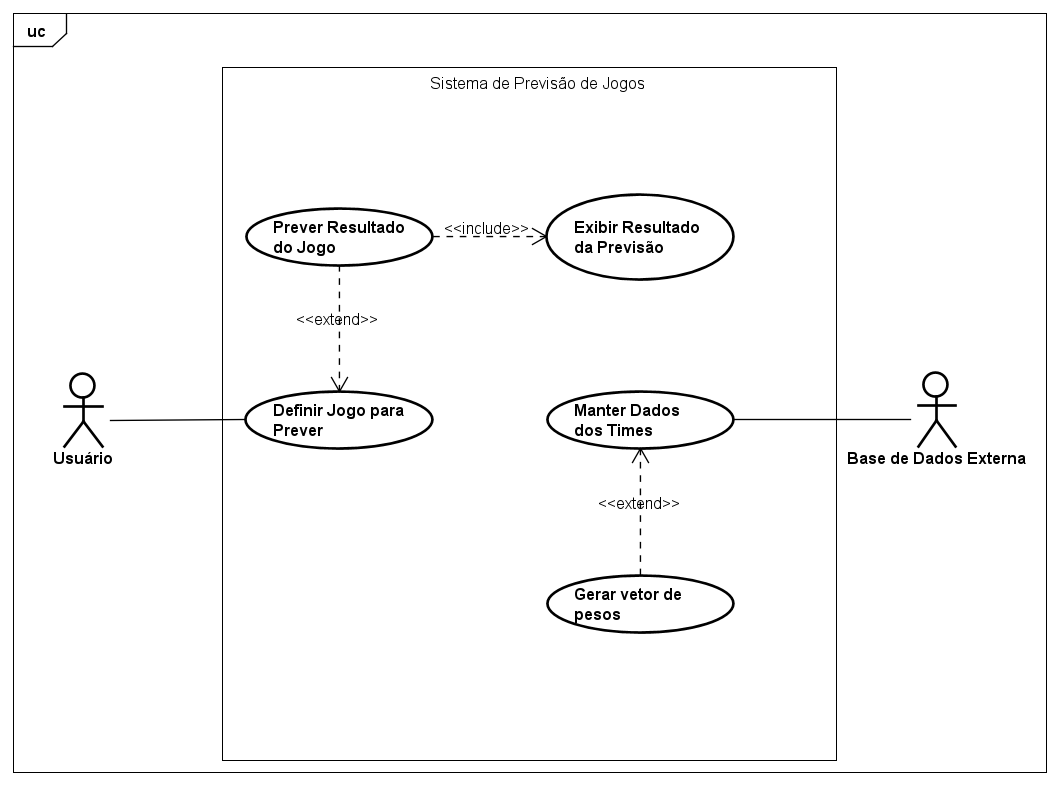
\includegraphics[width=.7\columnwidth]{img/Casos de Uso.png}
    \legend{Fonte: Desenvolvido pelos Autores (2020)}
    \label{fig:diagrama-casos-uso}
\end{figure}

\newpage

\subsection{Diagrama de Classes}
Nessa seção é mostrado o diagrama de classes. Os diagramas de classes representam a estrutura e relações entre as classes do sistema que servem de modelo para a instanciação dos objetos \cite{diagrama-classes}. A Figura \ref{fig:diagrama-classes} apresenta o Diagrama de Classes elencado no projeto.

\begin{figure} [H]
    \centering
    \caption{Diagrama de Classes}
    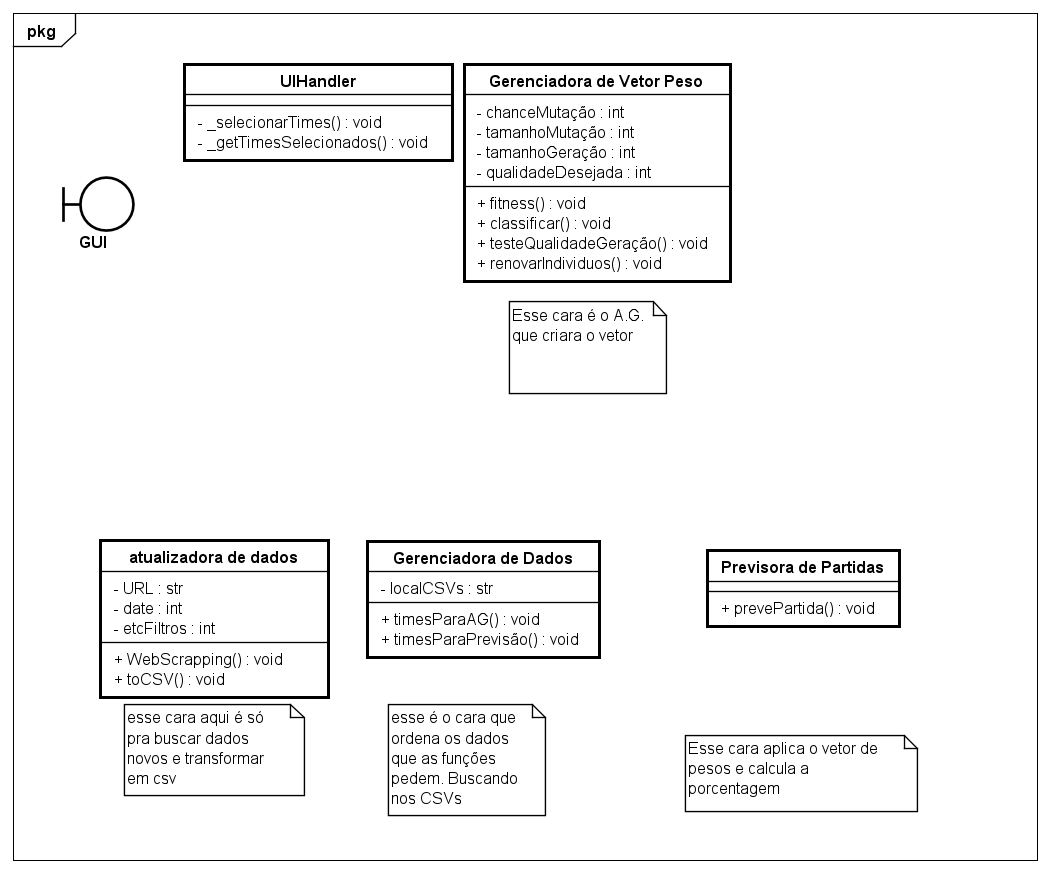
\includegraphics[width=.7\columnwidth]{img/Classes.png}
    \legend{Fonte: Desenvolvido pelos Autores (2020)}
    \label{fig:diagrama-classes}
\end{figure}


\subsection{Diagramas de Sequência}
Nesta seção são mostrados os diagramas de sequência. Seu principal objetivo é demonstrar em linhas de tempo quais são as interações entre os objetos de um determinado cenário representado pelo diagrama \cite{diagrama-sequencia}. As Figuras \ref{fig:diagrama-sequencia-definir-jogo}, \ref{fig:diagrama-sequencia-gerar-vetor}, \ref{fig:diagrama-sequencia-manter-dados} e \ref{fig:diagrama-sequencia-prever-jogo} apresentam os diagramas de sequência elencados no projeto.

\begin{figure}[H]
    \centering
    \caption{Diagrama de Sequência 1: Definir Partida para Prever}
    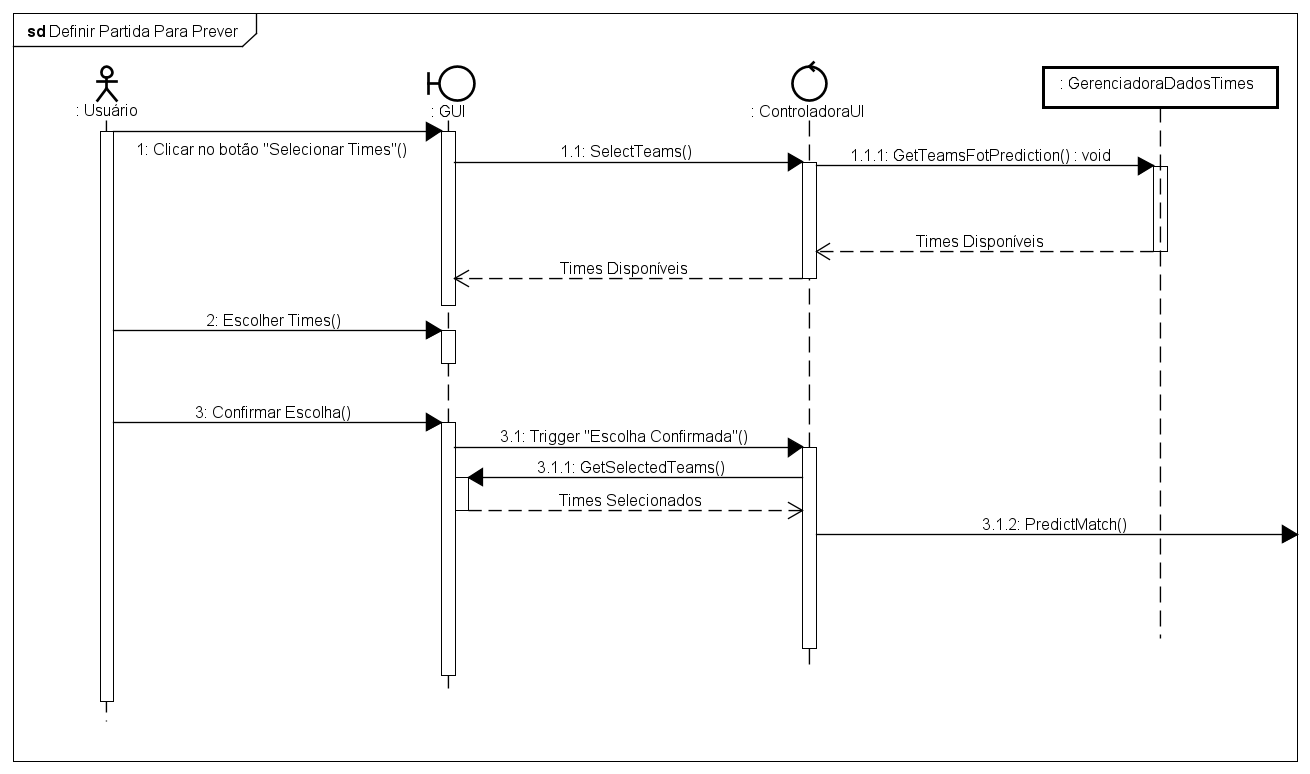
\includegraphics[width=.8\columnwidth]{img/Definir Partida Para Prever.png}
    \legend{Fonte: Desenvolvido pelos Autores (2020)}
    \label{fig:diagrama-sequencia-definir-jogo}
\end{figure}

\begin{figure}[H]
    \centering
    \caption{Diagrama de Sequência 2: Gerar Vetor de Pesos}
    \includegraphics[width=.7\columnwidth]{img/Algoritmo Genético.png}
    \legend{Fonte: Desenvolvido pelos Autores (2020)}
    \label{fig:diagrama-sequencia-gerar-vetor}
\end{figure}

\begin{figure}[H]
    \centering
    \caption{Diagrama de Sequência 3: Manter Dados dos Times}
    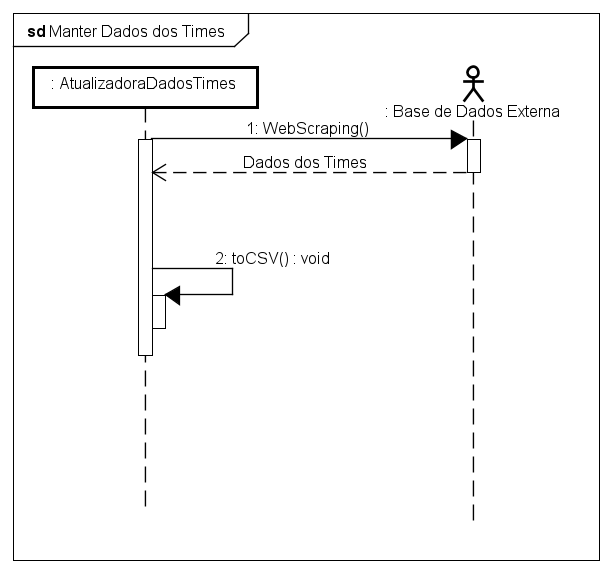
\includegraphics[width=.6\columnwidth]{img/Manter Dados dos Times.png}
    \legend{Fonte: Desenvolvido pelos Autores (2020)}
    \label{fig:diagrama-sequencia-manter-dados}
\end{figure}

\begin{figure}[H]
    \centering
    \caption{Diagrama de Sequência 4: Prever resultado da partida}
    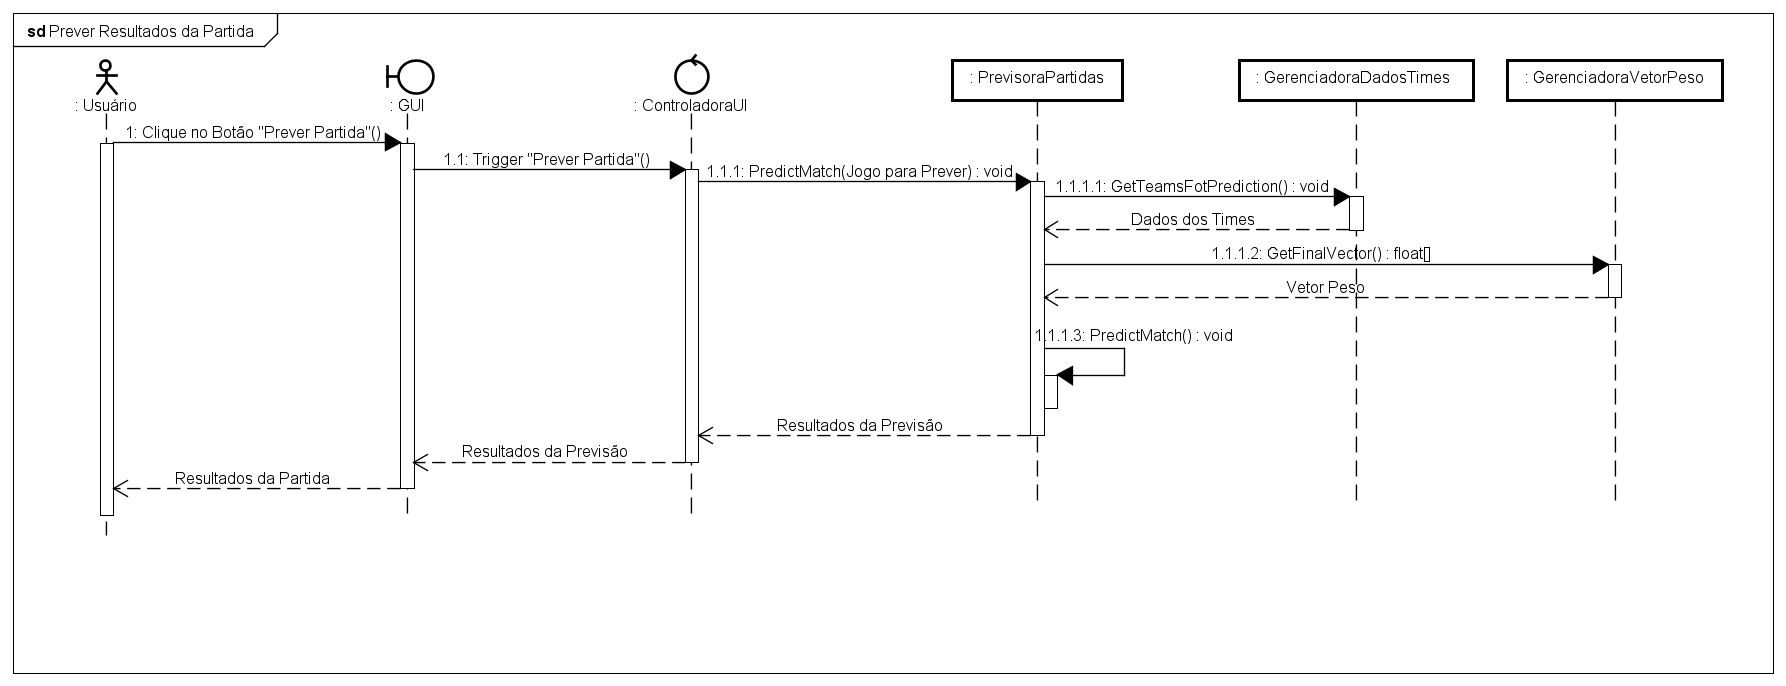
\includegraphics[width=.8\columnwidth]{img/Prever Resultados da Partida.png}
    \legend{Fonte: Desenvolvido pelos Autores (2020)}
    \label{fig:diagrama-sequencia-prever-jogo}
\end{figure}

\section{VALIDAÇÃO}
A validação do projeto irá consistir em obter os times que jogarão em partidas futuras, simular essas partidas no \textit{software} e anotar as previsões que ele realiza. Será colocado um cartaz detalhando as futuras partidas da NBA em mural no campus Gaspar do IFSC e toda vez que uma partida ocorresse, ele seria atualizado com a comparação entre o resultado real e o resultado previsto. Foi estabelecido como meta uma taxa de acerto de 70\%.

Outro método para realizar a validação deste trabalho é convidar estudantes do campus para usar o programa e avaliar suas experiências com a intuitividade da interface e as impressões que eles tiveram acerca das previsões realizadas pelo sistema. Isto seria mensurado através de um questionário, realizado posteriormente.

\chapter{CRONOGRAMA}

Nesta seção será apresentado o cronograma para o desenvolvimento deste projeto, e em seguida, uma explicação do que consiste cada etapa desse processo.

% Please add the following required packages to your document preamble:
% \usepackage{multirow}
% \usepackage{graphicx}
% \usepackage[table,xcdraw]{xcolor}
% If you use beamer only pass "xcolor=table" option, i.e. \documentclass[xcolor=table]{beamer}
\begin{table}[H]
\centering
\resizebox{\textwidth}{!}{%
\begin{tabular}{|c|c|c|c|c|c|c|c|c|c|c|c|c|c|c|c|}
\hline
\rowcolor[HTML]{EFEFEF} 
\cellcolor[HTML]{C0C0C0}                        & \multicolumn{11}{c|}{\cellcolor[HTML]{EFEFEF}2020}              & \multicolumn{4}{c|}{\cellcolor[HTML]{EFEFEF}2021} \\ \cline{2-16} 
\rowcolor[HTML]{EFEFEF} 
\multirow{-2}{*}{\cellcolor[HTML]{C0C0C0}Cronograma} & FEV & MAR & ABR & MAI & JUN & JUL & AGO & SET & OUT & NOV & DEZ & JAN & FEV & MAR & ABR \\ \hline
\cellcolor[HTML]{EFEFEF}Estudo Teórico      &   & X & X &   & X & X & X & X & X &   &   &   &   &   &   \\ \hline
\cellcolor[HTML]{EFEFEF}Testes              &   &   &   &   & X & X & X & X &   &   &   &   &   &   &   \\ \hline
\cellcolor[HTML]{EFEFEF}Conceituação        & X & X &   &   &   & X &   &   &   &   &   &   &   &   &   \\ \hline
\cellcolor[HTML]{EFEFEF}Análise de Sistemas &   &   &   &   &   &   & X & X &   &   &   &   &   &   &   \\ \hline
\cellcolor[HTML]{EFEFEF}Produção            &   &   &   &   &   &   &   &   &   & X & X & X & X & X &   \\ \hline
\cellcolor[HTML]{EFEFEF}Documentação        &   & X & X & X & X & X & X & X & X & X & X & X & X & X &   \\ \hline
\cellcolor[HTML]{EFEFEF}Apresentação        &   &   &   &   &   &   &   &   & X &   &   &   &   &   & X \\ \hline
\end{tabular}%
}
\caption{Cronograma}
\label{tab:cronograma}
\end{table}
%https://www.tablesgenerator.com/

\section{Estudo Teórico}
Nos períodos de estudo teórico, é feita uma análise das tecnologias disponíveis para selecionar quais serão propriamente utilizadas para o desenvolvimento do \textit{software}, e o estudo das ferramentas escolhidas, para já acostumar os membros da equipe a trabalharem com elas quando forem implementar o projeto em si.

\section{Testes}
Na fase de testes são criados protótipos usando as tecnologias selecionadas para o desenvolvimento do sistema descrito nesse projeto, com a finalidade de verificar a factibilidade do que está sendo proposto.

\section{Conceituação}
Na parte de conceituação foram planejados aspectos básicos do sistema final desejado, como o fluxo de código, e levantados os requisitos do sistema para a análise de sistemas poder ser realizada.

\section{Análise de Sistemas}
Nesta etapa do projeto foram feitas tanto a avaliação e correção dos requisitos levantados na fase de conceituação, quanto a criação dos diagramas UML (Figuras \ref{fig:diagrama-casos-uso} a \ref{fig:diagrama-sequencia-prever-jogo}).

\section{Produção}
Nesse período será feita a própria implementação do trabalho descrito neste documento, ou seja, esta seção do cronograma abrange os momentos em que será escrito código dentro do repositório do \textit{software}.

\section{Documentação}
Essa fase abrange a duração do projeto na qual foi ou será feita a descrição e documentação do sistema, e se estenderá até o final do desenvolvimento do \textit{software} e a escrita do artigo para a disciplina de Projeto Integrador II do IFSC. 

\section{Apresentação}
No estágio de apresentação será feita a exposição do projeto e o que foi realizado até o momento como parte das disciplinas de Projeto Integrador I e II do IFSC.

\newpage

\chapter{RESULTADOS ESPERADOS}
%Coisas para citar: maneira confiável de prever jogos, exemplo da eficiência de algoritmos genéticos, aprendizado das tecnologias
A princípio, espera-se que o \textit{software} desenvolvido ao longo deste trabalho, sirva como uma maneira relativamente confiável de obter previsões para resultados do primeiro quarto de partidas da NBA, além de atuar como possível referencial para futuros desenvolvedores com ideias similares a este projeto, como a precisão dos algoritmos genéticos para inferência de dados

Fora isso , é desejado que os membros da equipe desenvolvedora aprofundem seu conhecimento nas tecnologias aplicadas, como Python, interface gráficas, \textit{web scraping} e desenvolvimento de \textit{software} de uma maneira geral.

\bibliography{referencias}

%\begin{apendicesifsc}

%\chapter{Título do apêndice (se houver)}


%\end{apendicesifsc}

%\begin{anexosifsc}


%\chapter{Título do anexo (se houver)}


%\end{anexosifsc}

\end{document}